\documentclass{ximera}
%% handout
%% space
%% newpage
%% numbers
%% nooutcomes

%% You can put user macros here
%% However, you cannot make new environments

\graphicspath{{./}{firstExample/}{secondExample/}}

\usepackage{tikz}
\usepackage{tkz-euclide}
\usetkzobj{all}
\pgfplotsset{compat=1.7} % prevents compile error.

\tikzstyle geometryDiagrams=[ultra thick,color=blue!50!black]
 %% we can turn off input when making a master document

\outcome{Practice with improper integrals.}
\title{Deep Roots}
\author{Kirollos Masood}

\begin{document}
\begin{abstract}
In this activity, we will transcend the limits of man.
\end{abstract}
\maketitle

\begin{exercise}
	Show that
	\begin{align*}
		\sqrt{2}^{\sqrt{2}^{\sqrt{2}^{\ldots}}  }=2.
	\end{align*}
	
	Let's rephrase the problem using sequences. Define a sequence $\{c_n\}_{n=0}^{\infty}$ as follows.
	\begin{align*}
		c_0 &=\sqrt{2} \\
		c_1 &=\sqrt{2}^{c_0}=\sqrt{2}^{\sqrt{2}} \\
		c_2 &=\sqrt{2}^{c_1}=\sqrt{2}^{\sqrt{2}^{\sqrt{2}}} \\
		&\vdots \\
		c_{n+1}&=\sqrt{2}^{c_n} \\
		&\vdots
	\end{align*}
	So what we actually want to show is that $\lim_{n \to \infty} c_n = \answer[given]{2}$. We can start by just showing there is a limit. We can do this by showing our sequence is (monotonically) increasing and bounded above.
	
	\begin{remark}
		How do we show that $\{c_n\}$ is increasing? We start from the beginning. Is it true that $c_0 \leq c_1$? Well, we know that
		\begin{align*}
			b^p \leq b^q,
		\end{align*}
		assuming that $p\leq q$ and $b\geq 1$. In our situation, our base is $b=\sqrt{2}$, which is bigger than 1. Our exponents are $p=1$ and $q=\sqrt{2}$ and it is true that $p\leq q$. So the answer is yes. We've established that $\sqrt{2} \leq \sqrt{2}^{\sqrt{2}}$. Next, we should check if $c_1 \leq c_2$. That means we need to check if 
		\begin{align*}
			\sqrt{2}^{\sqrt{2}} \leq \sqrt{2}^{\sqrt{2}^{\sqrt{2}}}.
		\end{align*}
		That's true too! Our base is $b=\sqrt{2}$ again. But now, our exponents are $p=\sqrt{2}$ and $q=\sqrt{2}^{\sqrt{2}}$. Wait a minute; we just showed that $\sqrt{2} \leq \sqrt{2}^{\sqrt{2}}$ in the last step! We can repeat this process over and over again, which proves our sequence is increasing.
	\end{remark}
	
	\begin{remark}
		Next, we need to show our sequence is bounded above. We claim that the terms in our sequence never get bigger than 2. Once again, we start with our first term. We're in luck, because $c_0=\sqrt{2} \leq 2$. If you don't believe me, try squaring both sides. Okay, moving on, is it true that
		\begin{align*}
		c_{1}=\sqrt{2}^{\sqrt{2}} \leq 2?
		\end{align*}
		Try raising both sides to the power of $\sqrt{2}$. The left-hand side (LHS) becomes $\sqrt{2}^{\sqrt{2}*\sqrt{2}} = \sqrt{2}^2=2$. The right-hand side (RHS) becomes $2^{\sqrt{2}}$. And it is true that $2\leq 2^{\sqrt{2}}$. Now try playing this same game again and again for all the other terms. You'll quickly see that $c_n \leq 2$ no matter what $n$ we choose.
	\end{remark}
		
	Let's take a minute to step back and review what we've accomplished. So far, we've shown that $\{c_n\}$ is increasing and bounded above. That's enough to say the limit exists; let's call it $L$ for now. We still need to show that this limit has to be $2$.
	
	We already proved that $c_{n} \leq 2$. So take a limit on both sides. This tells us that
	\begin{align*}
	L = \lim_{n \to \infty} c_n \leq \answer[given]{2}.
	\end{align*}
	
	Here comes our greatest trick yet. We have the recursive relation
	\begin{align*}
	c_{n+1} = \sqrt{2}^{c_n}.
	\end{align*}
	Again, take a limit on both sides. On the LHS we get
	\begin{align*}
		\lim_{n \to \infty} c_{n+1} \answer[given]{L}
	\end{align*}. 
	On the RHS, we get
	\begin{align*}
	\lim_{n \to \infty} \sqrt{2}^{c_n} = \sqrt{2}^{ \lim_{n \to \infty} c_n} = \answer[given]{\sqrt{2}^L}.
	\end{align*}
	
	\begin{exercise}
		This means $L$ is a very special number. It satisfies the equation $L=\sqrt{2}^L$.
		
		\begin{image}
			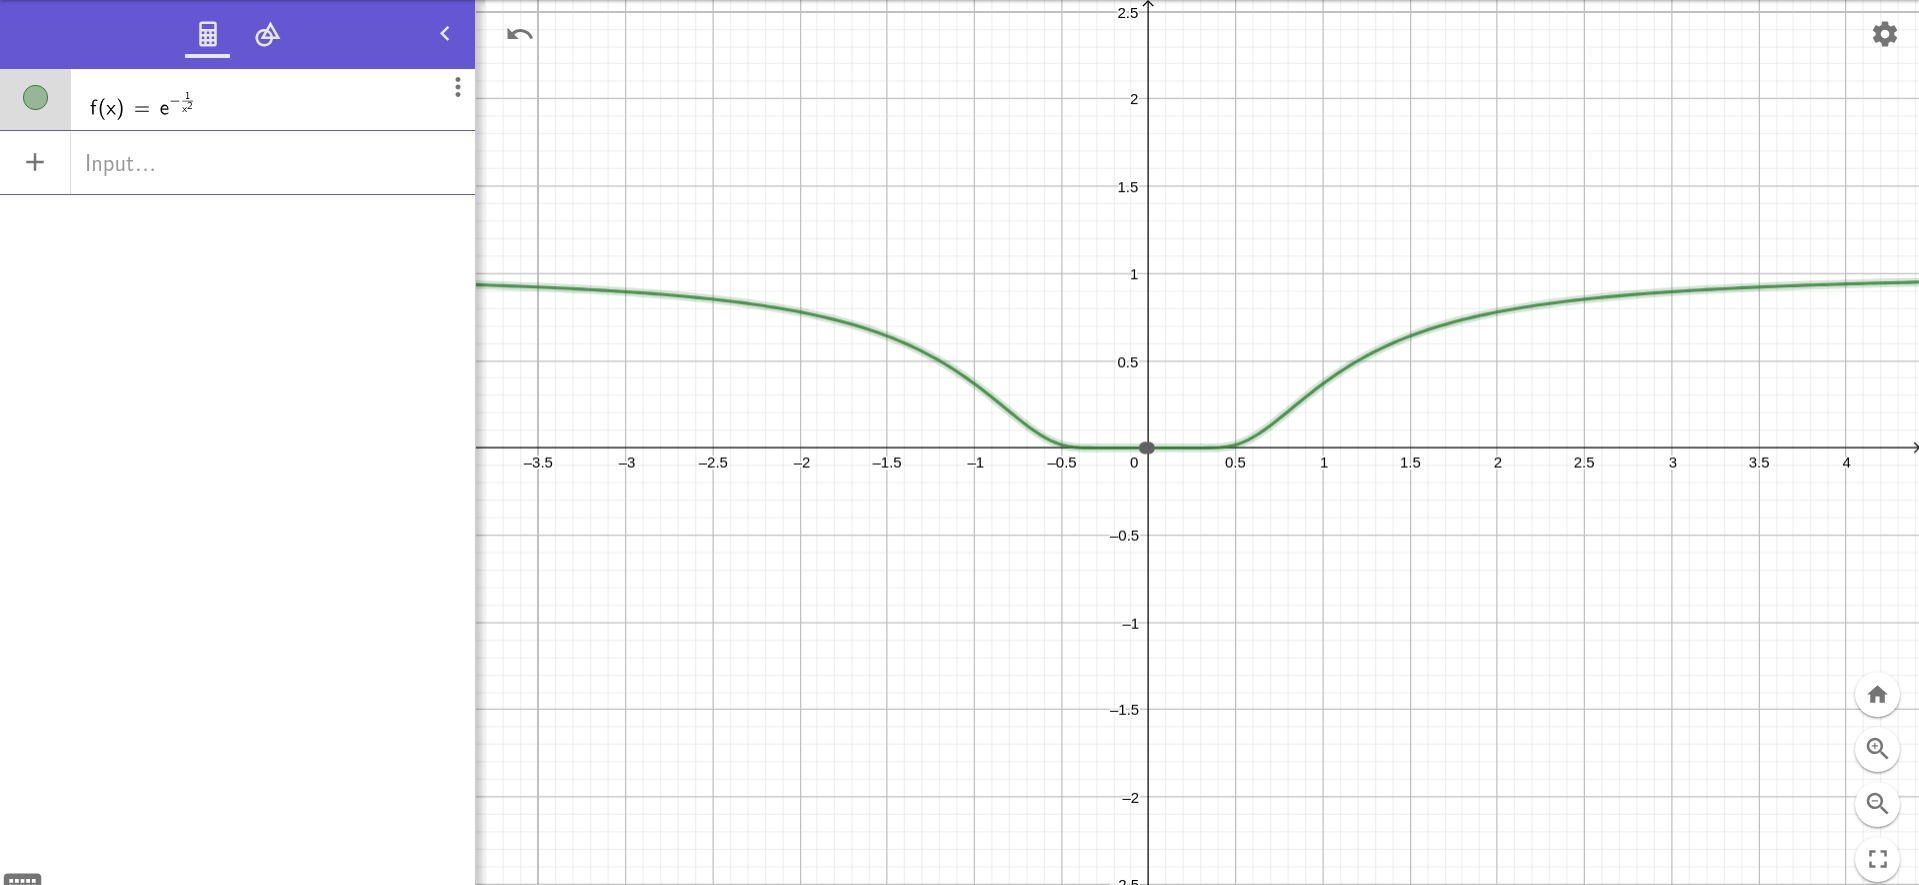
\includegraphics{graph.png}
		\end{image}
		
		From the graph above, we can see that the only solutions to the equation $x=\sqrt{2}^x$ are $x=2,4$. And we've already shown that $L \leq 2$. There's no doubt about it, $L=\answer[given]{2}$.
	\end{exercise}
	
\end{exercise}

\end{document}
